\documentclass{article}
\usepackage[utf8]{inputenc}
\usepackage[T1]{fontenc}
\usepackage{graphicx}
\usepackage{hyperref}
\usepackage{geometry}
\geometry{margin=1in}

\title{ACROTELERUTIC}
\date{Encyclopaedia Britannica (1771)}

\begin{document}
\maketitle

\section*{Historical source}
\textbf{Entry ID:} \texttt{entry-acrotelerutic-563} \\
\textbf{Volume ID:} 191253801 \\
\textbf{Character Count:} 705

\subsection*{Extracted Text}
ACROTELERUTIC, among ecdefalific writers, an appellation given to any thing added to the end of a plain; at the Gloria Patrir, or Doxology. GENERAL OTRISTERIA), in aestheticism, insall pedeals, usually without hates, secretly placed at the middle or two extremes of podmats or frontlipieces, ferrying to fopport the flames, see. It calls figuishes the figures placed as ornament on the tops of cherches, and the Pharp pointed that Band in ranges about flat buildings with rails and ballers.

Among ancient physicians, it figuified the larger ex-tremities of the body, as the heal, healths, and feet. It has also been rigid for the tips of the fingers and functions for the existence or proefices of bones.



\section*{Source record}
\begin{itemize}
\item \textbf{Dataset:} \texttt{NationalLibraryOfScotland/encyclopaedia\_britannica\_illustrated}
\item \textbf{Dataset Revision:} \texttt{309f765b1ecc83e0a7f7762e44b4a927a7555443}
\item \textbf{Page ID:} \texttt{britannica:309f765b1ecc83e0a7f7762e44b4a927a7555443:train:563} \\
  \textbf{Filename:} \texttt{page-0563-d12ce09577cd.jpg} \\
  \textbf{Row Index:} 563 \\
  \textbf{SHA256:} \texttt{d12ce09577cd595f...}
\end{itemize}

\begin{figure}[h]
\centering
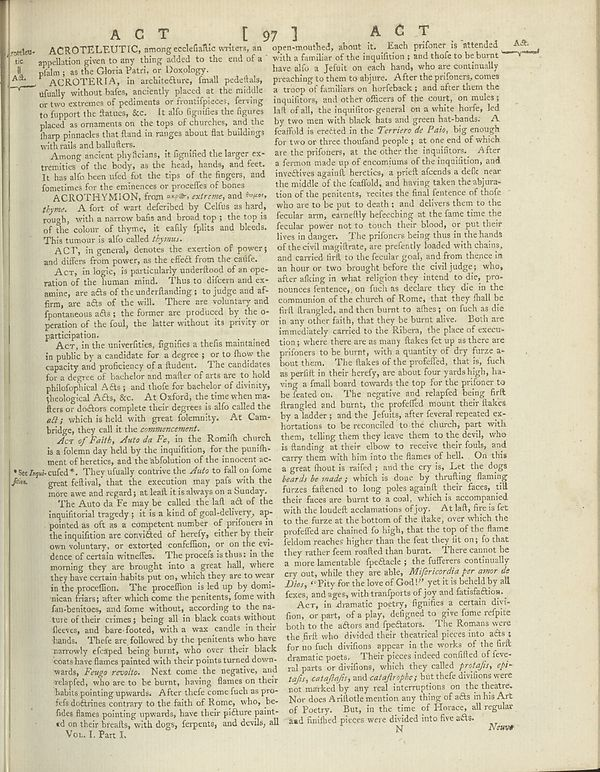
\includegraphics[width=0.85\textwidth]{../scans/page-0563-d12ce09577cd.jpg}
\caption*{Source scan: \texttt{page-0563-d12ce09577cd.jpg}}
\end{figure}

\end{document}
